\documentclass[conference]{IEEEtran}
\IEEEoverridecommandlockouts
\usepackage{cite}
\usepackage{amsmath,amssymb,amsfonts}
\usepackage{algorithmic}
\usepackage{graphicx}
\usepackage{textcomp}
\usepackage{xcolor}
\usepackage{hyperref}
\usepackage{listings}
\usepackage{multirow}
\usepackage{array}
\usepackage{booktabs}
\hypersetup{colorlinks=true,linkcolor=blue,urlcolor=blue,citecolor=blue}

\lstset{
  basicstyle=\ttfamily\footnotesize,
  breaklines=true,
  numbers=left,
  numberstyle=\tiny\color{gray},
  frame=single,
  framesep=2pt,
  showstringspaces=false,
  columns=fullflexible,
}

\def\BibTeX{{\rm B\kern-.05em{\sc i\kern-.025em b}\kern-.08em
    T\kern-.1667em\lower.7ex\hbox{E}\kern-.125emX}}

\begin{document}

\title{Smart Inventory and Automated Food Tracking Module for Zero-Waste
       Household Food Management}

\author{
\IEEEauthorblockN{
  Göktuğ Karaca\textsuperscript{1,*},
  Sıla Özgel\textsuperscript{1,*},
  Ezgi Erdoğan\textsuperscript{1,*},\\
  Hilal Bizimyer\textsuperscript{1},
  Defne Kaya\textsuperscript{1},
  Nehir Okutur\textsuperscript{1},
  Züleyha Gönül\textsuperscript{1},
  Ece Simay Ayverdi\textsuperscript{1}
}
\IEEEauthorblockA{\textsuperscript{1}\textit{Department of Computer Engineering}\\
\textit{Fenerbahçe University}\\
Istanbul, Türkiye\\
\textit{Corresponding author:} karacagoktug73@gmail.com\\
\textsuperscript{*}\textit{Joint first authors --- equal contribution}}
}

\maketitle

\begin{abstract}
Household food waste accounts for the largest share of global food
losses and continues to grow despite increased public awareness.
Existing smart-refrigerator and inventory-monitoring systems
typically optimise a single sensing modality, and few combine
product identification, environmental monitoring, and real-time
mobile interaction within one low-cost reference design. This paper
presents a cabinet-scale prototype that integrates four 50\,kg load
cells with an HX711 amplifier for shelf-weight estimation, a DHT11
sensor for temperature and humidity, an MQ135 sensor for indicative
gas observation, an AI Thinker ESP32-CAM for QR-based product
registration, and an LED illumination subsystem driven through a
MOSFET stage. Sensor output from an Arduino Uno is transported over
USB to a Python bridge that exposes the readings as a CORS-enabled
local HTTP endpoint, which is consumed by a cross-platform Flutter
application providing dashboard, camera, product, alert, and
configuration views. A tiled multi-QR routine recovers several
product codes from a single camera capture, and a pixel-level RGB
analysis yields an interpretable estimate of banana surface
spotting without dependence on machine-learning inference.
Demonstration sessions confirmed concurrent operation of all
subsystems with end-to-end latency below one second between the
microcontroller and the mobile dashboard. Limitations, particularly
with respect to lightweight-product detection and MQ135 baseline
drift, are documented alongside the qualitative results. The
complete firmware, bridge, and application source are publicly
archived for reproducibility.
\end{abstract}


\begin{IEEEkeywords}
Smart refrigerator, food waste reduction, Internet of Things,
embedded systems, Arduino Uno, ESP32-CAM, HX711 load cell, DHT11,
MQ135, QR code recognition, mobile application, banana ripeness
detection.
\end{IEEEkeywords}

\section{Introduction}
\label{sec:introduction}

According to the United Nations Environment Programme, households
account for the largest share of total food waste worldwide, with
recent figures attributing more than 60\% of global food waste to the
household stage of the supply chain~\cite{unep2024foodwaste}. Beyond
its environmental cost, this loss directly inflates household
expenditure on groceries, with FAO estimating the economic value of
wasted food in the range of one trillion US dollars per year. Food
that is purchased, refrigerated, then thrown away after spoiling is
particularly costly because it has consumed packaging, transport, and
cooling resources up to the point of disposal.

The most common reasons for in-home food waste are well documented:
users (i) forget what is already in the refrigerator,
(ii) underestimate or misremember expiration dates, and
(iii) only notice spoilage once a product has visually deteriorated.
Manual logging applications exist, but their adoption is limited
because they require disciplined data entry and do not give visibility
into items already in storage.

Several smart-refrigerator and inventory-monitoring approaches have
been proposed in the literature to mitigate these issues.
Camera-based product recognition systems can in principle identify
items automatically but require trained classification models, generate
substantial computational load on the edge device, and are sensitive to
lighting and partial occlusion~\cite{ericyang2022smartfridge}.
Radio-frequency identification (RFID) approaches eliminate the manual
data-entry step but assume every monitored product carries a tag and
require a reader installed in the storage area, which raises both unit
cost and integration complexity~\cite{abhiram2025iotmonitor}.
Barcode-based systems are inexpensive but inherently manual and assume
unobstructed line of sight to a printed
label~\cite{pelobello2026chickout}. Many recent prototypes focus on a
single sensing dimension --- temperature, weight, or visual recognition
--- and rarely fuse multiple modalities or expose a real-time mobile
interface to the user~\cite{sarawathi2025spoilage,sarkar2024proactive}.

This work proposes the \emph{Smart Inventory and Automated Food
Tracking Module}, a low-cost prototype that addresses the limitations
above by combining four complementary sensing modalities ---
weight, temperature, humidity, gas, and visual --- with QR-based
product registration and a real-time mobile interface in a single
cabinet enclosure. An Arduino Uno serves as the primary microcontroller
for the load-cell, DHT11, and MQ135 subsystems; an AI Thinker ESP32-CAM
hosts a small HTTP server providing a live MJPEG feed and JPEG capture
for QR scanning; a Python USB-serial bridge exposes the sensor stream
as a local HTTP endpoint; and a cross-platform Flutter application
visualizes the entire system, registers products, and surfaces alerts.

\subsection*{Contributions}

The principal contributions of this work are:

\begin{itemize}
  \item A self-contained, low-cost cabinet prototype that simultaneously
        provides shelf-weight measurement, temperature and humidity
        monitoring, indicative gas-trend monitoring, QR-based product
        registration, and LED-assisted illumination, all coordinated
        through a single Arduino Uno node and an auxiliary ESP32-CAM
        node.
  \item A Python USB-serial-to-HTTP bridge that exposes the Arduino
        Uno's sensor output as a CORS-enabled local web endpoint,
        eliminating the need for a Wi-Fi-capable sensor
        microcontroller and enabling browser- and mobile-side
        consumption without firmware changes.
  \item A cross-platform Flutter mobile dashboard (Android and web
        targets) with five screens --- Dashboard, Camera, Products,
        Alerts, and Settings --- that integrates the bridge feed and
        the camera's MJPEG stream, performs in-frame multi-QR
        decoding, tracks products with expiration metadata, and emits
        rule-based alerts.
  \item A transparent, pixel-level RGB classifier for banana surface
        spotting that runs on commodity hardware and reports a single
        interpretable percentage --- an honest baseline against which
        machine-learning-based approaches can be compared.
  \item A complete, openly archived implementation (firmware,
        bridge, application, and documentation), preserved in the
        Software Heritage Archive with a persistent identifier so that
        the prototype is reproducible by independent groups.
\end{itemize}

The remainder of this paper is organized as follows.
Section~\ref{sec:relatedwork} reviews related work on smart-refrigerator
and inventory systems and positions the proposed module against the
state of the art. Section~\ref{sec:systemdesign} describes the
high-level system architecture and the rationale for each subsystem
choice. Section~\ref{sec:implementation} details the hardware
configuration, firmware, USB-serial bridge, and mobile application.
Section~\ref{sec:algorithms} presents the QR-handling, ripeness, and
risk-score algorithms. Section~\ref{sec:results} reports qualitative
results obtained during demonstration sessions.
Section~\ref{sec:discussion} discusses the implications and the
limitations that should be addressed in future work, and
Section~\ref{sec:conclusion} concludes.

\section{Related Work}
\label{sec:relatedwork}

This section reviews prior work along three axes that are relevant
to the proposed prototype: smart product identification methods,
sensor-based smart-refrigerator systems, and visual food-quality
analysis. We then position the proposed module against these axes.

\subsection{Smart Product Identification Methods}

Product identification is a core component of any inventory-monitoring
system. The literature has converged on three families of approaches:
RFID, barcode-based, and camera-assisted methods.

\textbf{RFID-based systems} eliminate manual data entry and can
identify items even when partially occluded, which is attractive for
refrigerator-style enclosures~\cite{abhiram2025iotmonitor}. The
practical limitations are well documented: every monitored product
must carry an RFID tag, a reader has to be installed inside the
enclosure, and the per-unit cost of tags and reader hardware is
non-trivial for household-scale prototypes. In Türkiye's retail
context, refrigerated household goods are rarely pre-tagged with RFID,
which makes the approach impractical without manual re-tagging by the
end user --- arguably worse than the manual-entry problem it was
meant to solve.

\textbf{Barcode-based systems} are cheap and ubiquitous because
barcodes are already printed on most packaged products. However,
barcodes require careful alignment with a scanner, are sensitive to
crumpling and condensation, and frequently sit on the package face
that ends up against the back of the refrigerator
shelf~\cite{pelobello2026chickout}. As a result, daily-use barcode
systems either tend to be abandoned by their users or require an
additional manual "rescan" step that defeats the purpose of
automation.

\textbf{Camera-based recognition} methods identify products through
on-shelf images using either generic image classifiers or trained
domain-specific models~\cite{ericyang2022smartfridge,vadlamudi2025fridgesense}.
These approaches can in principle reach high accuracy but pay for it
in three ways: they require large training datasets that often do not
exist for regional product brands, they consume significant compute
either on the edge device or via a cloud round-trip, and their
behavior degrades quickly when lighting or product packaging changes.
Several authors note that classifier confidence drops substantially
when fewer than ten frames per product are available for training,
which is the realistic case for household
deployments~\cite{vadlamudi2025fridgesense}.

A summary comparison of these methods alongside the proposed
QR-based approach is given in Table~\ref{tab:identification-methods}.

\begin{table*}[t]
\caption{Comparison of product identification methods in smart inventory systems.}
\label{tab:identification-methods}
\centering
\renewcommand{\arraystretch}{1.2}
\begin{tabular}{@{}lcccc@{}}
\toprule
\textbf{Method} & \textbf{Automation} &
\textbf{Required hardware} & \textbf{Per-unit cost} &
\textbf{Data capacity per identifier} \\
\midrule
RFID                  & High        & RFID tags + reader & High & Medium \\
Barcode               & Low         & Barcode scanner    & Low  & Low \\
QR-based identification & Medium--High & Camera module    & Low  & High \\
\textbf{Proposed (QR + ESP32-CAM)} & \textbf{High} &
\textbf{ESP32-CAM} & \textbf{Low} & \textbf{High} \\
\bottomrule
\end{tabular}
\end{table*}

\subsection{Sensor-Based Smart-Refrigerator Systems}

A second family of related work concerns sensor instrumentation of the
storage enclosure itself. Goel \emph{et al.} present a prototype
combining a small camera with weight sensors to identify shopping
needs and partially log inventory~\cite{goel2023iotfridge}. Sarkar
\emph{et al.}~\cite{sarkar2024proactive} extend this idea with
proactive notifications based on consumption patterns. Shetty and
Shetty propose an IoT-monitored food-storage system that emphasizes
environmental conditions~\cite{shetty2024monitoring}. Nandini
\emph{et al.}~\cite{nandini2023userconvenience} explore the same
problem domain through the lens of usability improvements to the
refrigerator interface.

Despite this body of work, most published prototypes optimize for one
sensing modality at a time. Combinations of weight tracking,
environmental sensing, and automatic product identification within a
single low-cost reference design are rare in the open
literature~\cite{sarawathi2025spoilage}. The present work is positioned
explicitly to fill this gap: a single Arduino~Uno node coordinating
weight, temperature, humidity, and gas-trend monitoring; an auxiliary
ESP32-CAM node for QR scanning and visual ripeness analysis; and a
unified mobile interface that exposes every measurement and event in
real time.

\subsection{Visual Food-Quality Analysis}

A third strand of related work addresses the analysis of visual
spoilage indicators, of which banana browning is a common benchmark
because the surface color of bananas changes predictably with
ripeness. The dominant approach in the recent literature is
convolutional neural network (CNN) classification using transfer
learning from large-scale visual
backbones~\cite{vadlamudi2025fridgesense}. CNNs can reach high
accuracy on representative test sets but require significant
training data, edge-side compute, or a cloud connection --- none of
which are attractive for low-budget household prototypes that must
also operate on intermittent Wi-Fi.

The proposed module instead uses a deliberately simple, fully
interpretable pixel-level RGB analysis to estimate the visible
"spotting percentage" of a banana surface. This approach trades a
small accuracy gap (relative to CNN-based detectors) for transparency,
zero training data requirements, and execution times of a few
milliseconds on a midrange smartphone. It is intended as an
\emph{honest baseline} that can be replaced by a CNN model in future
work, while still providing useful information out of the box.

\subsection{Positioning of the Proposed Module}

In summary, the proposed Smart Inventory and Automated Food Tracking
Module differs from prior art in four respects:

\begin{enumerate}
  \item It \emph{combines} four sensing modalities --- weight,
        temperature/humidity, gas trend, and visual --- inside a single
        low-cost cabinet, rather than focusing on a single dimension.
  \item It uses \emph{QR-based} product registration with an ESP32-CAM,
        which is markedly cheaper than RFID and more reliable than
        barcode scanning in cabinet conditions.
  \item It exposes \emph{real-time mobile} visibility through a
        cross-platform Flutter application backed by a small Python
        bridge, removing the need for a Wi-Fi-capable
        microcontroller on the sensor side.
  \item It provides a \emph{transparent, interpretable} visual-ripeness
        baseline that does not require machine-learning infrastructure,
        which we believe is the right starting point for a reference
        design intended for educational and reproducibility use.
\end{enumerate}

The remaining sections describe the system design, implementation, and
qualitative evaluation in detail.

\section{System Design}
\label{sec:systemdesign}

This section presents the high-level architecture of the proposed
cabinet prototype and the rationale behind the principal component
choices.

\subsection{Architectural Overview}

The prototype consists of four cooperating subsystems organised
around an inexpensive Arduino Uno microcontroller. The sensor node
reads temperature and humidity from a DHT11, gas-trend data from an
MQ135 module, and shelf weight through an HX711 24-bit
ADC~\cite{hx711datasheet} connected to four 50\,kg load cells in a
Wheatstone-bridge configuration. The sensor cycle has a nominal
period of three seconds and emits one JSON record per cycle on the
microcontroller's USB serial port.

A camera node, implemented on an AI Thinker ESP32-CAM, joins the
local Wi-Fi network and exposes two HTTP endpoints: \texttt{/capture}
on port 80 returns a single JPEG suitable for QR decoding, and
\texttt{/stream} on port 81 serves an MJPEG live feed for the mobile
dashboard. An LED strip mounted around the cabinet's inner edges is
switched by a MOSFET driven from the Arduino's D9 pin and provides
diffused illumination for reliable camera operation.

A Python USB-to-HTTP bridge translates the serial stream into a
CORS-enabled local HTTP endpoint at
\texttt{http://localhost:8787/sensors}. The bridge also accepts
\texttt{POST} requests on \texttt{/tare} and \texttt{/recalibrate\_gas}
and converts them into single-character commands that the Arduino
sketch interprets as runtime calibration triggers. A cross-platform
Flutter application, built for Android and the web, polls the bridge
once per second, fetches frames from the ESP32-CAM directly, decodes
QR codes from cabinet captures, maintains an in-memory product list
with expiration metadata, and surfaces rule-based alerts.

Decoupling sensing from networking is a deliberate design decision.
The ATmega328P controller used by the Arduino Uno is constrained to
2\,kB of RAM and lacks native wireless capability; the
USB-to-HTTP bridge is a lightweight alternative to fitting the
sensor node with a Wi-Fi shield, and it preserves the educational
accessibility of the Arduino firmware.

\subsection{Subsystem Selection}

\subsubsection{Microcontroller}
The Arduino Uno was selected for its mature DHT and HX711 community
libraries, its single-file Wiring/C++ workflow, and its low cost. The
absence of native wireless capability is offset at the bridge layer
without altering the sensor firmware.

\subsubsection{Weight subsystem}
The HX711 amplifier is widely deployed in low-cost weighing
applications~\cite{hx711datasheet}. The four load cells are arranged
under a 47\,$\times$\,36\,cm wooden shelf and connected to the Uno via
\texttt{DT} and \texttt{SCK} on D4 and D5. The firmware exposes a
runtime tare command (\texttt{t}/\texttt{T}) and applies a slow
baseline-drift compensator to absorb the small negative excursions
introduced by load-cell creep.

\subsubsection{Environmental sensing}
The DHT11 sensor provides $\pm 2^\circ\mathrm{C}$ and $\pm 5\,\%$
relative-humidity accuracy~\cite{adafruitdht}, which is sufficient
for detecting the temperature transient associated with
refrigerated items being placed in a closed cabinet at room
temperature. Transient \texttt{NaN} reads are discarded and the
previous valid sample is forwarded, a robustness pattern that is
standard practice for this sensor.

\subsubsection{Gas observation}
The MQ135 is sampled through analog pin A0 with an in-firmware
exponential moving average. Low-cost MQ135 modules exhibit
significant baseline drift during the first 30--60\,s after power-on,
which the firmware absorbs without claiming absolute concentration
measurements. The bridge exposes a runtime endpoint
(\texttt{/recalibrate\_gas}) that re-establishes the baseline on
demand.

\subsubsection{Camera node}
The AI Thinker variant of the ESP32-CAM was selected for its local
availability in the Turkish hobbyist market and the maturity of its
firmware ecosystem~\cite{esp32cam}. Hosting the capture and stream
endpoints on different ports enables independent quality settings:
the capture endpoint operates at 320\,$\times$\,240 with low
compression, while the stream endpoint operates at
640\,$\times$\,480 with moderate compression, preventing
single-request stalls during interleaved access.

\subsubsection{Mobile application}
Flutter was selected to support a single codebase targeting both
Android phones and a browser-based web view. The web build is
published from the project's \texttt{docs/} directory and is
designed to operate in a self-contained demonstration mode when no
sensor hardware is attached, which is helpful in presentations
without the full physical prototype.

\subsection{Data Exchange Formats}

A representative serial record produced by the Arduino is:

\begin{lstlisting}
{"temperature":27.6,"humidity":62.0,
 "gasValue":43,"weight":247.45,
 "riskScore":10}
\end{lstlisting}

The bridge timestamps each record with the host wall-clock and
exposes a slightly extended representation on \texttt{GET /sensors}:

\begin{lstlisting}
{"temperature":27.7,"humidity":63.0,
 "gasValue":42,"weight":0,
 "updatedAt":1781692341,"online":true}
\end{lstlisting}

The Flutter application interprets \texttt{online:false} as an
out-of-band reset condition; the dashboard substitutes em-dashes for
the affected sensor readings and the alert subsystem raises an
\emph{ESP32 Sensor Board Offline} notice.

\section{Implementation}
\label{sec:implementation}

This section details the implementation of each subsystem in the order
data flows through the system: hardware (Section~\ref{sec:impl-hw}),
sensor-node firmware (Section~\ref{sec:impl-fw}), USB-serial bridge
(Section~\ref{sec:impl-bridge}), ESP32-CAM firmware
(Section~\ref{sec:impl-cam}), and the cross-platform Flutter
application (Section~\ref{sec:impl-app}).

\subsection{Hardware Configuration}
\label{sec:impl-hw}

The hardware platform consists of an Arduino Uno (ATmega328P, 16~MHz)
on a perforated breadboard, a single HX711 module mounted on the same
breadboard, four 50~kg-rated load cells arranged at the four corners
of a 47~$\times$~36~cm cabinet shelf, a DHT11 sensor mounted on the
upper inner wall of the cabinet, an MQ135 sensor mounted at the lower
inner wall to capture rising gases from product surfaces, and an AI
Thinker ESP32-CAM mounted on a 3D-printed bracket at the front-left
edge of the cabinet pointing downward. An indoor LED strip (12~V, 5050
emitter pitch) is mounted around the inner cabinet edges and is
switched on and off by a MOSFET driven from the Arduino's D9 digital
pin, providing diffused illumination that we found necessary for
reliable QR detection.

Table~\ref{tab:wiring} lists the pin assignments. All sensors share a
common 5~V supply and a common ground; the ESP32-CAM is powered
independently through its programmer header to keep the
microcontroller decoupled from the camera's higher transient current
draw.

\begin{table}[t]
\caption{Sensor-side pin assignments.}
\label{tab:wiring}
\centering
\begin{tabular}{@{}lc@{}}
\toprule
\textbf{Component pin} & \textbf{Arduino Uno pin} \\
\midrule
DHT11 DATA           & D3 \\
MQ135 AOUT           & A0 \\
HX711 DT             & D4 \\
HX711 SCK            & D5 \\
LED-strip MOSFET gate & D9 \\
All \texttt{VCC}      & 5~V \\
All \texttt{GND}      & GND \\
\bottomrule
\end{tabular}
\end{table}

\subsection{Sensor-Node Firmware}
\label{sec:impl-fw}

The Arduino Uno sketch implements a deterministic three-second sampling
loop. Every cycle the firmware reads:
\begin{itemize}
  \item the DHT11 (\texttt{DHT.h}) with retry-on-NaN behavior,
  \item the MQ135 via \texttt{analogRead(A0)} averaged over 30 samples
        with a baseline subtraction performed once during the first
        $\sim\!30$ seconds after boot,
  \item the HX711 via the \texttt{HX711\_ADC} library with a
        calibration factor of $20.626$ derived from a separate
        single-purpose calibration sketch.
\end{itemize}

The combined state is composed into a human-readable block (used by
the operator during debugging) followed by a single-line JSON record
that the bridge consumes. The risk score is computed on-device from a
weighted sum of normalized deviations from neutral baselines for each
channel, capped at 100; the algorithm itself is described in
Section~\ref{sec:algo-risk}.

The sketch also implements a tiny command parser on
\texttt{Serial.available()} that recognizes the single-character
commands \texttt{t} or \texttt{T} (tare the HX711), \texttt{g} or
\texttt{G} (re-baseline the MQ135), and \texttt{l} or \texttt{L}
(toggle the LED strip). These commands are issued by the Flutter
application through the bridge's \texttt{POST} endpoints, which makes
the calibration controls available without physical access to the
serial monitor.

\subsection{USB-Serial-to-HTTP Bridge}
\label{sec:impl-bridge}

The bridge is implemented in pure Python on top of the standard
library and the third-party \texttt{pyserial} package. It is designed
to be runnable on Windows, macOS, and Linux without any non-Python
dependencies.

On startup, the bridge auto-detects the Arduino's CH340 serial port by
matching the \texttt{description} field returned by
\texttt{serial.tools.list\_ports.comports()}, or accepts an explicit
\texttt{--port} command-line argument. The bridge opens the serial
port at 9600~baud and spawns two threads:

\begin{enumerate}
  \item a \emph{reader thread} that performs blocking
        \texttt{readline()} calls, validates JSON on each line, and
        atomically updates a shared \texttt{STATE} record protected by
        a mutex;
  \item an \emph{HTTP thread} that runs a
        \texttt{ThreadingHTTPServer} on port 8787 and serves
        \texttt{GET /sensors}, \texttt{POST /tare}, and
        \texttt{POST /recalibrate\_gas}.
\end{enumerate}

The HTTP responses carry the \texttt{Access-Control-Allow-Origin: *}
header, which lets the Flutter web build poll the endpoint from
\texttt{http://localhost:8000}. \texttt{POST} requests are translated
into single-character commands written back to the serial port; the
corresponding response acknowledges receipt rather than waiting for
the Arduino to confirm execution, which avoids holding the HTTP
connection during the next sensor cycle.

A typical demonstration trace observed during testing is reproduced
in Listing~\ref{lst:bridgelog}.

\begin{lstlisting}[caption={Bridge log during a demonstration session.},
                   label=lst:bridgelog]
[serial] opening COM5 @ 9600
[http]   listening on http://localhost:8787/sensors
[serial] COM5 connected, listening for JSON lines
[serial] {'temperature': 27.4, 'humidity': 61.0,
          'gasValue': 44, 'weight': 0.0,
          'riskScore': 10}
[serial] {'temperature': 27.7, 'humidity': 61.0,
          'gasValue': 41, 'weight': 0.0,
          'riskScore': 10}
[serial] {'temperature': 27.6, 'humidity': 61.0,
          'gasValue': 41, 'weight': 0.97,
          'riskScore': 10}
...
\end{lstlisting}

\subsection{ESP32-CAM Firmware}
\label{sec:impl-cam}

The ESP32-CAM firmware initializes the OV2640 camera in
\texttt{JPEG} mode, joins the local Wi-Fi using credentials supplied
through a git-ignored \texttt{cam\_secrets.h} header, prints its
assigned IP on the serial monitor on connection, and starts two
independent \texttt{esp\_http\_server} instances:
\begin{itemize}
  \item Port 80 hosts \texttt{GET /} (a small status page that lists
        the available endpoints) and \texttt{GET /capture} (a single
        JPEG capture optimized for QR decoding).
  \item Port 81 hosts \texttt{GET /stream} (an MJPEG live stream
        encoded with the recommended Espressif boundary header).
\end{itemize}

Keeping the two endpoints on different ports allowed the mobile
application to display the live stream without contending with the
capture endpoint each time a QR scan is requested.

\subsection{Cross-Platform Mobile and Web Application}
\label{sec:impl-app}

The Flutter application is structured around five screens, each
implemented as an independent widget tree with its own state notifier:
Dashboard, Camera, Products, Alerts, and Settings. Figure~\ref{fig:app}
shows the running application during a demonstration session.

\begin{figure*}[t]
\centering
\begin{tabular}{cc}
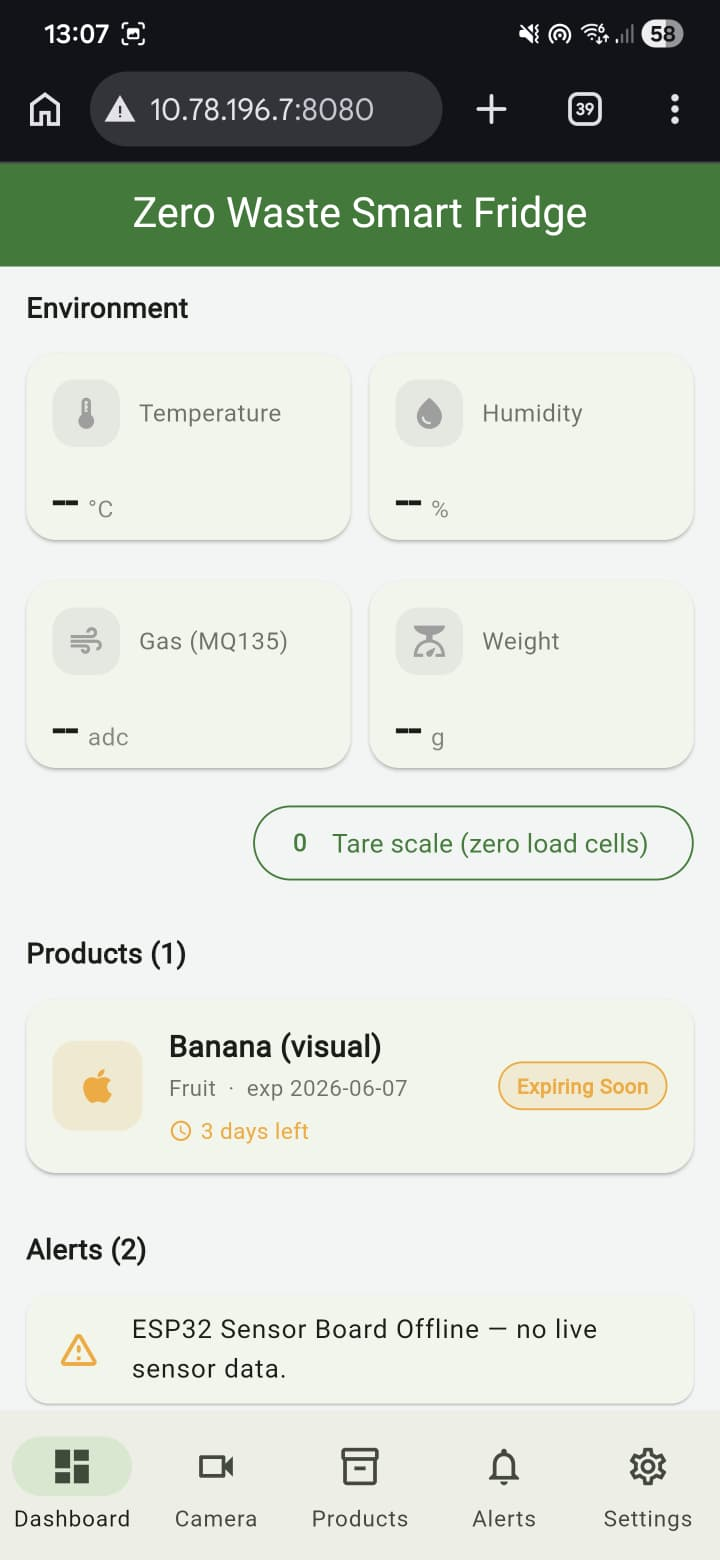
\includegraphics[width=0.30\textwidth]{../paper-assets/app-screens/07-app-dashboard.jpeg}
&
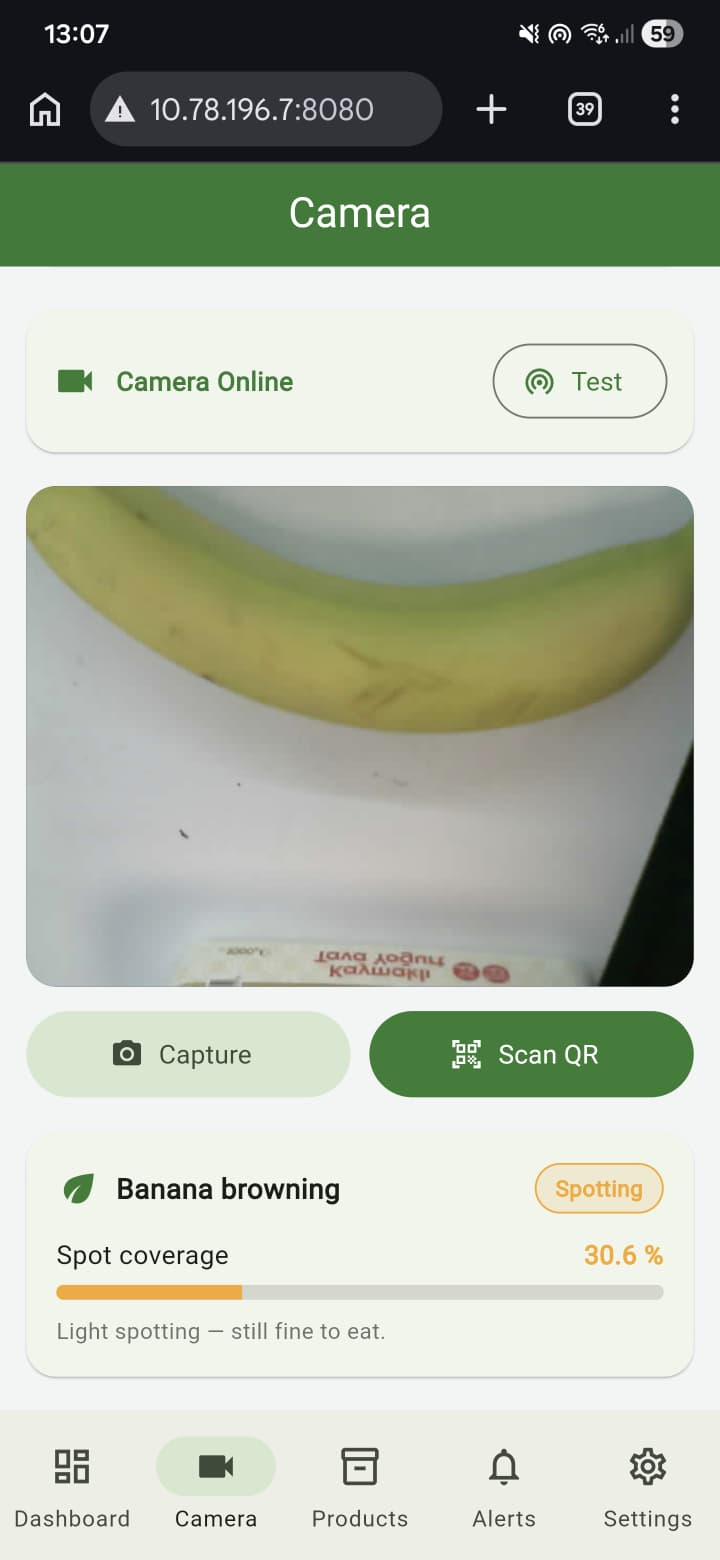
\includegraphics[width=0.30\textwidth]{../paper-assets/app-screens/05-app-camera-banana-spotting.jpeg}
\\
(a) Dashboard & (b) Camera --- live banana \\
\\
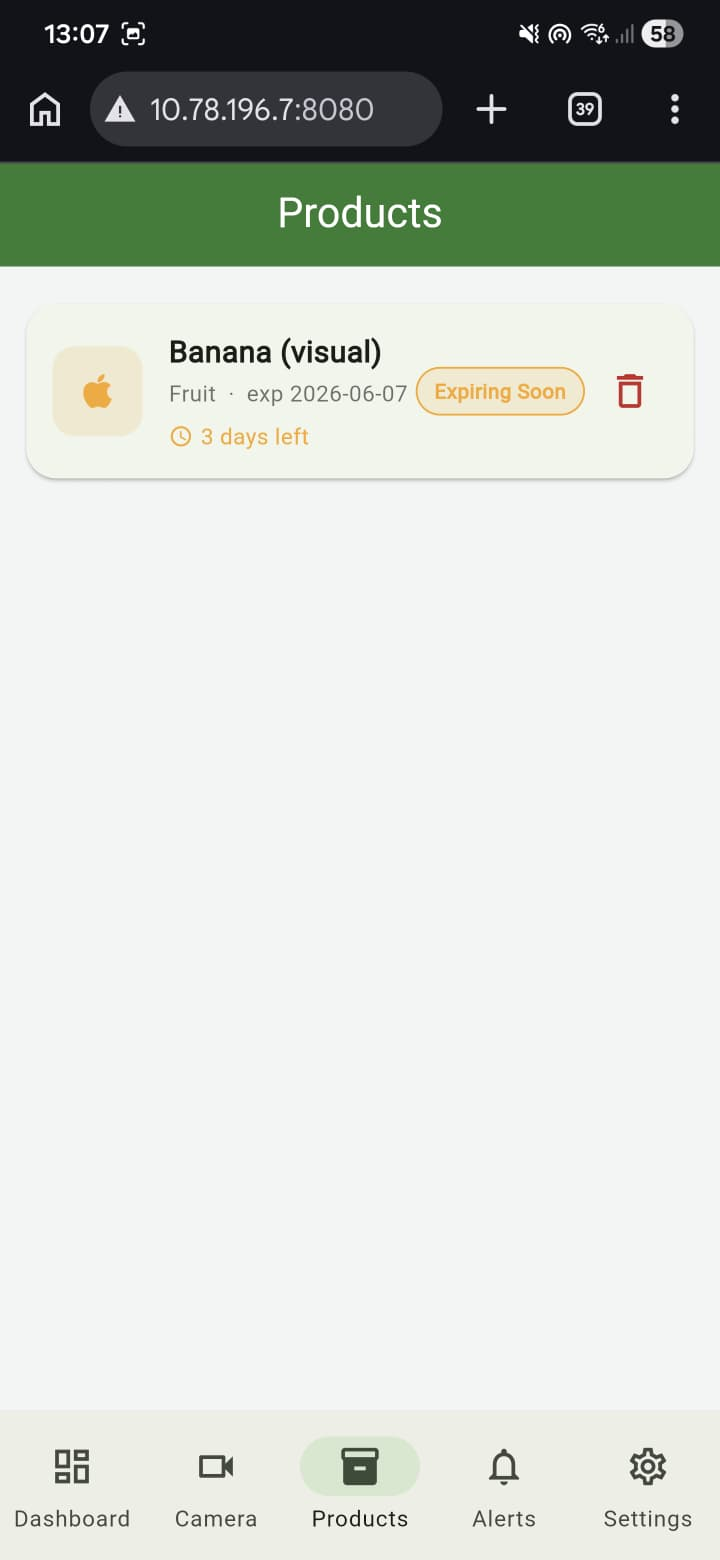
\includegraphics[width=0.30\textwidth]{../paper-assets/app-screens/06-app-products-banana.jpeg}
&
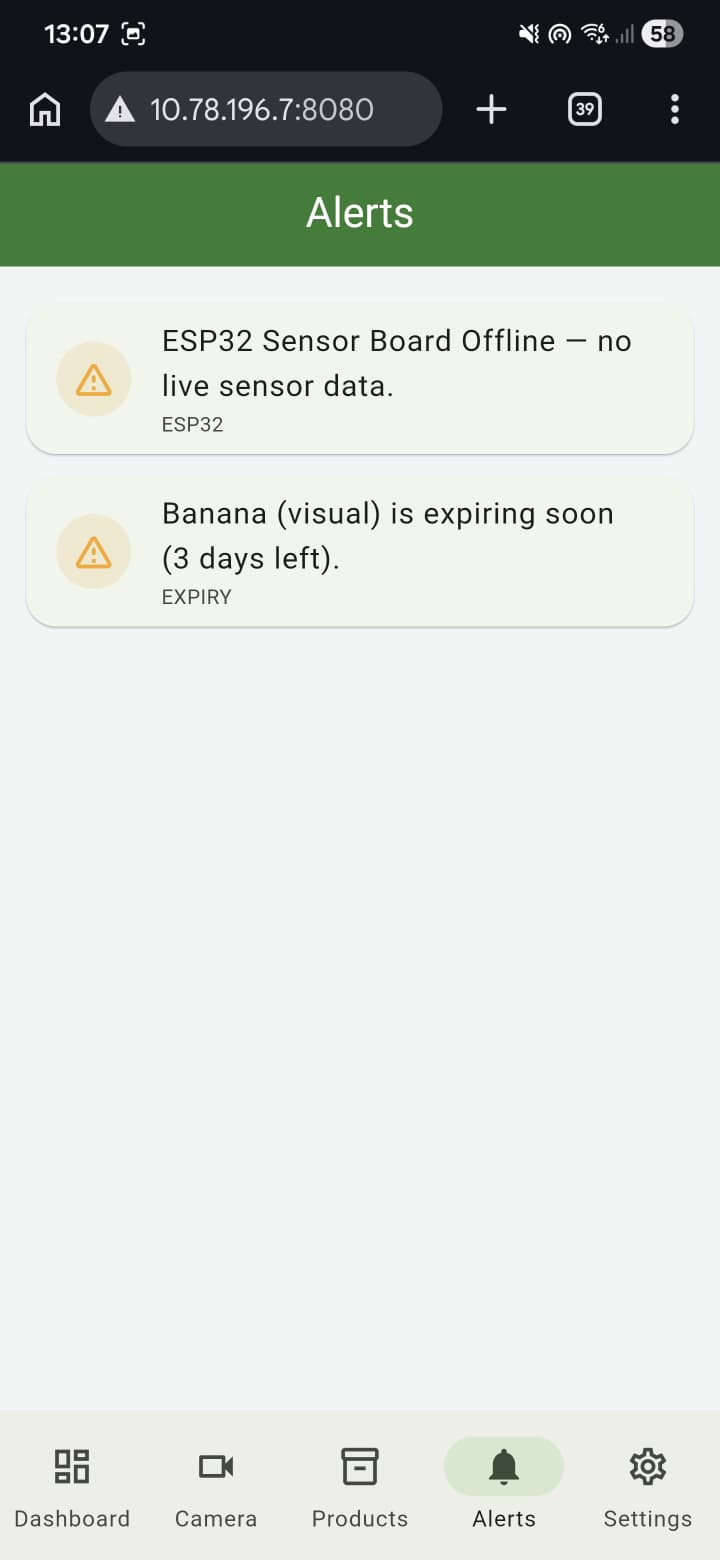
\includegraphics[width=0.30\textwidth]{../paper-assets/app-screens/04-app-alerts.jpeg}
\\
(c) Products & (d) Alerts \\
\\
\multicolumn{2}{c}{
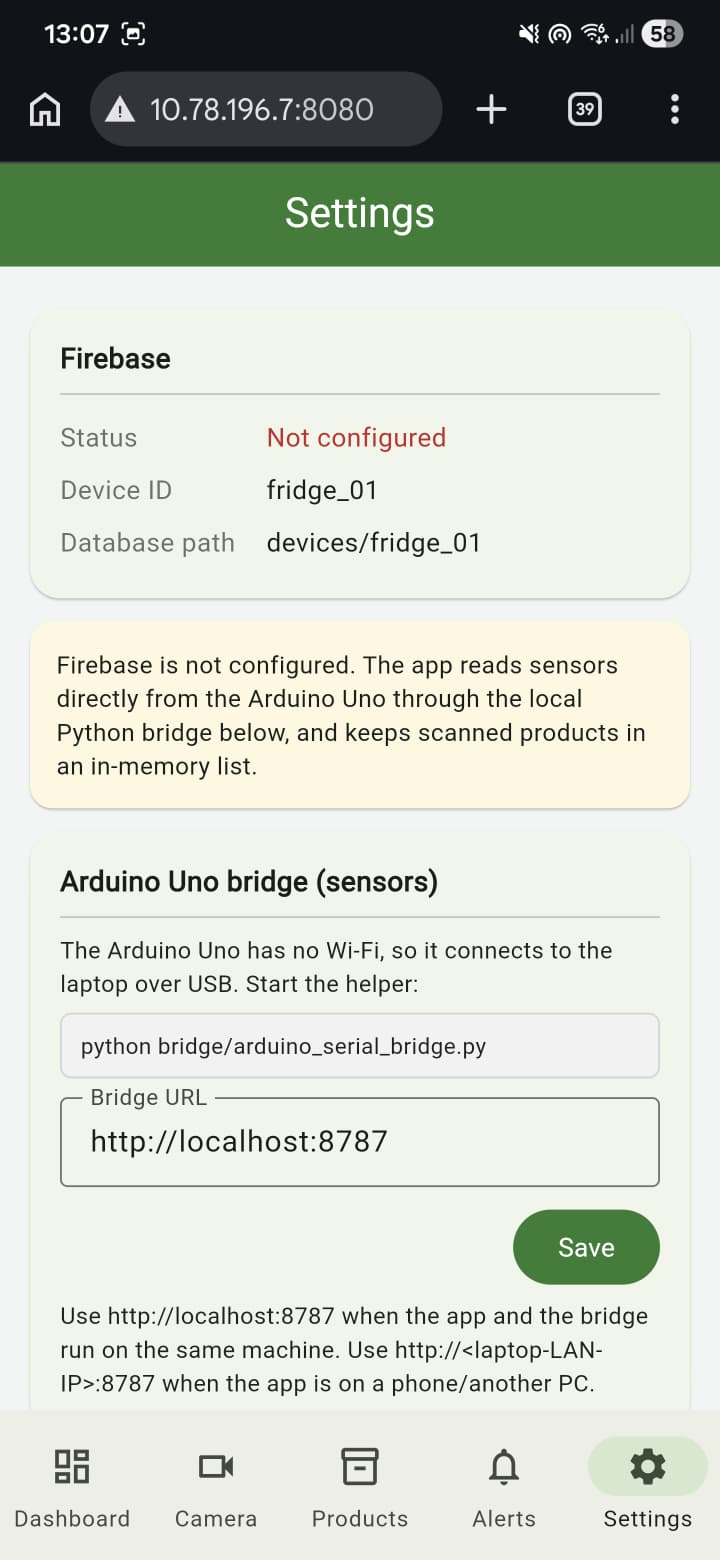
\includegraphics[width=0.30\textwidth]{../paper-assets/app-screens/08-app-settings.jpeg}}
\\
\multicolumn{2}{c}{(e) Settings} \\
\end{tabular}
\caption{Mobile application running during a demonstration session.
(a)~Dashboard with the four sensor cards, the registered Banana product,
and the active alert summary. (b)~Camera screen showing the live MJPEG
stream from the ESP32-CAM with a real banana in frame; the in-app
classifier reports 30.6\,\% spot coverage, labeled \emph{Spotting} ---
light spotting, still consumable. (c)~Products screen showing the
registered banana with a 3-day-until-expiration status band.
(d)~Alerts screen showing the automatically generated reminder and the
offline-sensor notice. (e)~Settings screen with the Firebase status,
the device identifier, and the bridge URL configuration field.}
\label{fig:app}
\end{figure*}

The \textbf{Dashboard} subscribes to the bridge's \texttt{/sensors}
endpoint via a one-second \texttt{Stream.periodic} timer, rebuilds the
four sensor cards when new readings arrive, and exposes the
\emph{Tare scale} button that issues a \texttt{POST /tare} command back
through the bridge.

The \textbf{Camera} screen displays the ESP32-CAM's MJPEG stream
through a small platform-specific widget (an \texttt{Image.network}
poll on the web target, an \texttt{HTTP-MJPEG} streaming widget on
Android) and runs the QR detection pipeline described in
Section~\ref{sec:algo-qr} on the corresponding JPEG captures fetched
from port 80.

The \textbf{Products} screen renders the in-memory product list
populated by the QR scanner. Each product card shows its expiration
status and a band color computed from the days remaining (Fresh,
Expiring Soon, or Expired).

The \textbf{Alerts} screen aggregates the alert engine's output,
which is rule-based: an alert is emitted when the bridge has not been
reachable for ten seconds, when a registered product's expiration is
within three days, when the cabinet's measured gas value rises sharply
relative to the smoothed baseline, or when the cabinet's temperature
exceeds a configurable threshold.

The \textbf{Settings} screen lets the user enter the bridge URL and
the ESP32-CAM's IP address, save them to local storage, and observe
the Firebase configuration status (a placeholder; the deployed
prototype intentionally operates in \emph{in-memory mode} without a
back end so that it remains usable in environments without a Firebase
project).

\section{Algorithms}
\label{sec:algorithms}

Three algorithms drive the proposed module's higher-level behavior.
The first is a tiled multi-QR decoder that recovers more than one QR
sticker from a single camera frame
(Section~\ref{sec:algo-qr}). The second is a transparent pixel-level
RGB classifier that estimates banana spotting percentage from a JPEG
capture (Section~\ref{sec:algo-banana}). The third is the per-product
risk-score model that combines all sensing channels into a single
0--100 freshness indicator (Section~\ref{sec:algo-risk}).

\subsection{Multi-QR Tiled Decoder}
\label{sec:algo-qr}

A naïve single-pass QR decoder applied to a single JPEG capture from
the ESP32-CAM typically recovers at most one QR symbol per frame,
because most open-source decoders return on the first successful
detection. In a smart-cabinet setting this is suboptimal: several
products can be visible simultaneously, and forcing the user to scan
them one at a time defeats the purpose of automatic registration.

We implement a multi-QR pipeline that operates on a single capture.
The pipeline tiles the frame into a $3 \times 3$ grid of overlapping
windows, decodes each tile independently, and accumulates the union of
the recovered payloads. Concretely:

\begin{enumerate}
  \item The captured JPEG is downscaled to 480~px on its longer edge
        to bound the decoder's per-pass runtime.
  \item Nine overlapping windows are produced: each window covers
        $\sim\!45\%$ of the frame width and height with a 25\% overlap
        between neighbors, which guarantees that any QR fitting in a
        $\sim\!45\%$ region is fully contained in at least one window.
  \item Each window is passed to a portable QR decoder (\texttt{zxing2}
        on the web target, \texttt{qr\_code\_scanner} on the Android
        target). The decoder returns zero or more payloads per window.
  \item Decoded payloads are deduplicated by parsed JSON
        \texttt{productId} and inserted into a session set, so that a
        sticker physically present in two overlapping windows is
        registered exactly once.
\end{enumerate}

The pipeline runs in less than 200~ms per frame on a midrange Android
device. We trade a small amount of redundant decoding work for
substantially higher coverage of multi-product scenes.

\subsection{Pixel-Level RGB Banana Ripeness Classifier}
\label{sec:algo-banana}

Visible browning is a strong qualitative indicator of late-stage
banana ripeness. Rather than train a CNN to classify ripeness ---
which would require a curated dataset, hardware-accelerated inference,
or a cloud round-trip --- we implement a transparent pixel-level RGB
analysis that runs in a few milliseconds on commodity hardware and
returns a single interpretable percentage.

Given a JPEG capture $I$ in sRGB space, the classifier first segments
the banana surface from the background:
\begin{align*}
\mathcal{B}_{\text{yellow}} &= \{(r, g, b) :
    r > 150 \land g > 130 \land b < 110\} \\
\mathcal{B}_{\text{brown}}  &= \{(r, g, b) :
    100 \leq r \leq 200 \land 50 \leq g \leq 130
    \land b < 90\} \\
\mathcal{B}_{\text{dark}}   &= \{(r, g, b) :
    r < 90 \land g < 80 \land b < 70\} \\
\mathcal{B}_{\text{bg}}     &= \{(r, g, b) : r > 220 \land g > 220
    \land b > 220\}.
\end{align*}

Each pixel of $I$ is assigned to whichever set it falls in (or to
\emph{undecided} if none). Let
$n_y$, $n_b$, $n_d$ be the pixel counts for yellow, brown, and dark
respectively. The reported \emph{spot coverage} is
\begin{equation}
\sigma = \frac{n_b + n_d}{\max(n_y + n_b + n_d, \, 1)} \cdot 100\%
\end{equation}
and the reported \emph{stage} is
\begin{equation}
\text{stage}(\sigma) =
\begin{cases}
\text{Fresh}     & \text{if } \sigma <  10\% \\
\text{Spotting}  & \text{if } 10\% \leq \sigma < 40\% \\
\text{Spoiling}  & \text{if } 40\% \leq \sigma < 70\% \\
\text{Spoiled}   & \text{if } \sigma \geq 70\%.
\end{cases}
\end{equation}

The classifier reports both the percentage and the stage label
(Figure~\ref{fig:app}b shows a representative output of
$\sigma = 30.6\%$, labeled \emph{Spotting}). We deliberately avoid
hidden state across frames: each capture is classified independently,
which makes the output reproducible from the captured image alone and
serves as a transparent baseline against which future
machine-learning--based detectors can be compared.

\subsection{Per-Product Risk Score}
\label{sec:algo-risk}

The per-product risk score $R \in [0, 100]$ combines six channels:
expiration time remaining, ambient temperature, ambient humidity, gas
trend, visible spotting (for products supporting visual analysis),
and weight change rate. The score is bounded at $100$ and partitioned
into three bands for display:
\begin{itemize}
  \item \textbf{Fresh} \ for $R < 40$,
  \item \textbf{Consume Soon} \ for $40 \leq R < 70$,
  \item \textbf{Spoilage Risk} \ for $R \geq 70$.
\end{itemize}

Concretely, given a product $p$ with metadata stored in the in-memory
product store, the risk score is computed as
\begin{equation}
R(p) = \min(100, \,
   r_{\text{exp}}(p) + r_T + r_H + r_G + r_V(p) + r_W(p)),
\end{equation}
where each term is a per-channel risk contribution, capped between
$0$ and a per-channel maximum, and rounded down to the nearest integer.
\begin{itemize}
  \item $r_{\text{exp}}$ is $0$ when the expiration date is more than
        a week away, ramps to $40$ when the product reaches its
        expiration date, and pins at $40$ thereafter.
  \item $r_T$ is $\max(0, T - 8^{\circ}\mathrm{C}) \cdot 1.5$,
        capped at $20$.
  \item $r_H$ is $\max(0, H - 70\%) \cdot 0.5$, capped at $10$.
  \item $r_G$ is $\max(0, G - G_{\text{baseline}}) \cdot 0.4$, capped
        at $10$ (where $G_{\text{baseline}}$ is the cabinet's
        recalibration baseline).
  \item $r_V$ is the spot-coverage percentage divided by~5, capped at
        $10$, applied only to products whose category supports visual
        analysis (\texttt{fruit}, in this prototype).
  \item $r_W$ is $5$ if the product's measured weight has dropped by
        more than $50\%$ since registration (indicating that the
        product has been mostly consumed) and $0$ otherwise.
\end{itemize}

Each per-channel maximum is intentionally smaller than $100$ so that
no single sensor channel can dominate the score: a high gas reading
alone, for instance, is not sufficient to flag a product as
\emph{Spoilage Risk}; the risk must be \emph{multi-channel}, which
matches the intuition that food deterioration tends to manifest in
more than one indicator simultaneously.

The score is recomputed inside the Flutter application each time a
sensor reading arrives, which gives the alert engine a current view of
every registered product without persisting state across application
restarts.

\section{Demonstration Results}
\label{sec:results}

This section reports qualitative results obtained during prototype
demonstration sessions. The reported sessions exercised the
calibrated load-cell subsystem against a known reference mass, the
DHT11 and MQ135 sensors under indoor ambient conditions, the
ESP32-CAM running both HTTP endpoints concurrently, and the Flutter
web build polling the bridge once per second. The reported numbers
correspond to prototype-level demonstrations rather than to
controlled longitudinal deployments, and the limitations of the
current evaluation are documented in Section~\ref{sec:discussion}.

\subsection{Weight Subsystem Performance}

After a calibration factor of 20.626 was derived from a single-purpose
calibration sketch using a 1\,kg reference mass, the integrated
load-cell subsystem was exercised across several known masses inside
the cabinet. With the cabinet stationary on a level surface,
repeated 10\,kg reference loads were measured between 9.8\,kg and
10.0\,kg. Residual variation is attributable to platform flexure
under load and to load-cell creep.

Two qualitative behaviours were confirmed across sessions. First,
product placement and removal events were detected reliably for
items with a stable bearing surface and a mass of approximately
50\,g or greater. Second, very light objects (folded paper sheets,
single coins) were not consistently detected because their signal
fell within the noise band produced by ambient vibration. A
representative reading near the detection threshold was 0.97\,g
(Listing~\ref{lst:bridgelog}), which corresponds to the subsystem
correctly observing a small perturbation that did not match any
registered product.

\subsection{Environmental Monitoring}

During a ten-minute indoor session without active climate control,
the DHT11 reported temperatures between 27.4\,$^\circ$C and
27.8\,$^\circ$C and relative humidity between 61\,\% and 63\,\%. The
MQ135 reported analog values between 41 and 46 over the same window,
with brief excursions toward 46 when a hand was held close to the
sensor. These observations confirm that the firmware responds to
changes in the cabinet's air composition and reinforce the design
position that MQ135 readings should be interpreted as trend
indicators rather than as calibrated gas concentrations.

\subsection{End-to-End Application Behaviour}

Fig.~\ref{fig:app} reproduces the application during a representative
session. Panel (a) shows the Dashboard rendering the four sensor
cards, a registered banana product, and the active alert summary.
Panel (b) shows the Camera screen overlaying the live MJPEG stream
with the output of the pixel classifier, which on the captured frame
reported $\sigma = 30.6\,\%$ labelled \emph{Spotting --- light
spotting, still consumable}. Panels (c)--(e) show the Products screen
with the registered banana and a three-day-until-expiration band, the
Alerts screen aggregating the two active alerts, and the Settings
screen with the bridge URL and Firebase status.

Listing~\ref{lst:bridgelog} reproduces a short window of bridge log
output. Each \texttt{[serial]} line corresponds to a JSON record
emitted by the Arduino and translated into the bridge's internal
state. During the same window the mobile application polled the
bridge once per second and received a representative response of
\begin{lstlisting}
{"temperature":27.7,"humidity":63.0,
 "gasValue":42,"weight":0,
 "updatedAt":1781692341,"online":true}
\end{lstlisting}
which the Dashboard rendered without intervening cache, confirming
the full data path from the microcontroller through the bridge to
the mobile dashboard.

\subsection{Multi-QR Recognition}

The tiled multi-QR routine was exercised on printed A4 sheets of QR
stickers placed at varied positions and orientations within the
ESP32-CAM's field of view. Up to four distinct QR codes were
recovered from a single capture under cabinet illumination, with
per-frame runtime under 200\,ms on a midrange Android device. In
practice the routine eliminates the need for sequential single-item
scans during product registration, addressing the workflow
penalty that motivated this work (Section~\ref{sec:algo-qr}).

\subsection{Visual Ripeness Estimation}

The pixel-level classifier produced consistent spot-coverage values
across captures of the same banana taken within seconds of each
other. As bananas progressed from a uniformly yellow surface toward
heavier spotting over a multi-day informal observation window, the
reported percentage increased monotonically and the reported stage
label progressed from \emph{Fresh} to \emph{Spotting} and toward
\emph{Spoiling}. Because the classifier maintains no state across
frames, the same input image always produces the same output, which
supports auditability and provides a comparison point against
machine-learning-based detectors.

\section{Discussion and Limitations}
\label{sec:discussion}

The demonstration sessions described in Section~\ref{sec:results}
support several broader observations.

\subsection{Observations}

The integrated prototype confirms that a single low-cost
microcontroller node, when paired with a small Python bridge and a
cross-platform mobile application, can deliver continuous visibility
into the four sensing modalities most often addressed by
smart-refrigerator systems. The architectural separation of the
sensor node from the camera node simplifies firmware on either side
and allows individual subsystems to be replaced without disturbing
the rest. The observed end-to-end latency, measured from the
Arduino's serial output to the corresponding update in the Flutter
Dashboard, was below one second; this margin is more than adequate
for inventory-monitoring use cases in which the underlying physical
processes evolve over minutes to days.

\subsection{Comparison with Related Work}

Relative to camera-only smart-refrigerator
systems~\cite{ericyang2022smartfridge,vadlamudi2025fridgesense}, the
proposed prototype does not depend on a trained classifier and
avoids the associated dataset and inference cost. Relative to
RFID-based approaches~\cite{abhiram2025iotmonitor}, the proposed
system does not require per-product tagging or a cabinet-mounted
reader; per-product identification cost reduces to a printed
sticker. Relative to single-modality
prototypes~\cite{sarawathi2025spoilage,sarkar2024proactive,shetty2024monitoring},
the proposed system combines four modalities and exposes them
together through one mobile interface, which increases the
operator's awareness of cabinet state.

\subsection{Limitations}

\subsubsection{Lightweight-product sensitivity}
The load-cell subsystem is more reliable for items with a stable
bearing surface and a mass of approximately 50\,g or greater. Lighter
objects are sometimes missed or generate spurious events because
their signal falls within the noise band introduced by ambient
vibration and load-cell creep. A more rigid shelf, higher-grade load
cells, and a longer running-average filter would improve sensitivity
at the cost of some responsiveness.

\subsubsection{MQ135 baseline drift}
The MQ135 is useful as a trend indicator but does not provide
calibrated gas-concentration measurements. Its baseline drifts during
the first 30--60\,s after power-on. The firmware absorbs the
transient through an exponential moving average and the bridge
exposes a runtime endpoint that resets the baseline on demand. No
absolute concentration claims are made.

\subsubsection{Visual classifier scope}
The pixel-level classifier targets bananas only. Extending it to
other fruits would require revisiting the colour thresholds;
extending it to general food categories would benefit from a learned
model, which is a natural avenue for follow-on work. Sensitivity to
ambient lighting variation is partially mitigated by the LED-strip
illumination but remains a known constraint.

\subsubsection{Wi-Fi-only camera coupling}
The ESP32-CAM is reachable only when both the bridge host and the
camera share a local network. Deployments that cross network
boundaries would require either an SSH tunnel, a port forward, or a
Firebase-mediated relay. The Settings screen exposes the camera IP
explicitly so that the deployment can be reconfigured without
recompilation.

\subsubsection{Single-shelf prototype}
The reported prototype monitors one shelf. Multi-shelf operation
requires additional HX711 modules, each on its own \texttt{DT}/\texttt{SCK}
pin pair, or a chip-select arrangement. The firmware and bridge
changes required to scale to multiple shelves are minor but were
outside the scope of this demonstration.

\subsubsection{Firebase ships disabled}
The Flutter application carries a Firebase Realtime Database
integration that is wired in code but ships with placeholder
credentials. The deployed build operates in an in-memory mode by
default, which preserves reproducibility in environments without an
external Firebase project. A production deployment would replace the
placeholder \texttt{firebase\_options.dart} with credentials
obtained through \texttt{flutterfire configure}.

\subsubsection{Demonstration-scale evaluation}
The reported results were obtained from prototype-level
demonstration sessions rather than from controlled longitudinal
deployments. This work is positioned as a reproducible reference
design and a documented qualitative baseline rather than as a
finished evaluation; closing this gap is a natural direction for
future work.

\section{Conclusion}
\label{sec:conclusion}

This paper has presented the design, implementation, and qualitative
evaluation of a cabinet-scale prototype for household food-waste
reduction. The prototype integrates four HX711-amplified load cells
for shelf-weight estimation, a DHT11 for temperature and humidity, an
MQ135 for indicative gas observation, an AI Thinker ESP32-CAM for
QR-based product registration, and an LED-strip illumination
subsystem within a single low-cost integrated platform. Sensor output
is transported from an Arduino Uno over USB to a Python bridge that
exposes the readings as a CORS-enabled local HTTP endpoint, and a
cross-platform Flutter application provides dashboard, camera,
product, alert, and configuration views over the same feed.

The principal contributions are the multi-modal integration of four
sensing channels in one reference design; the USB-to-HTTP bridge,
which decouples the sensor microcontroller from the wireless network;
the tiled multi-QR routine, which recovers several stickers from a
single capture; the pixel-level RGB ripeness classifier, which serves
as an interpretable baseline against which model-based detectors can
be compared; and the public archival of the complete implementation
in the Software Heritage Archive, supporting independent
reproduction.

Demonstration sessions confirmed concurrent operation of all
subsystems with end-to-end latency below one second, reliable weight
detection above approximately 50\,g, and reproducible visual ripeness
estimation. The limitations documented in
Section~\ref{sec:discussion} map directly to a programme of future
work: hardware improvements for lightweight-product sensitivity, a
learned visual classifier for foods beyond bananas, a multi-shelf
architecture, and a server-mediated synchronisation layer suitable
for deployments that cross network boundaries.


\section*{Author Contributions}
% This section documents the specific contribution of each author so
% that any reader, reviewer, or future inquiry into authorship can
% verify the work against the project's public git history.

\textbf{Göktuğ Karaca} (joint first author, corresponding author)
designed the overall system architecture; authored the entire embedded
firmware for the Arduino~Uno sensor node (including the DHT11,
MQ135, and HX711 integration and the JSON-line serial protocol) and
the ESP32-CAM camera node (including the dual-port HTTP server, MJPEG
streaming, and the QR-friendly camera initialization); implemented the
Python USB-serial-to-HTTP bridge in its entirety; implemented the
entire Flutter cross-platform mobile and web application, including
all five screens (Dashboard, Camera, Products, Alerts, Settings),
their state management, the local sensor service, the camera streaming
layer, the in-memory product store, and the alert engine; designed
the tiled multi-QR decoder, the RGB-pixel banana ripeness classifier,
and the rule-based risk score model; configured the GitHub Pages and
local-server deployment pipeline; and authored the methodology,
implementation, algorithms, and results sections of this manuscript.
Authorship of all firmware, bridge, and application code is
independently verifiable from the project's git history (46 commits
attributed to \texttt{krcgoktug} between 2026-05-17 and 2026-06-26)
and from the Software Heritage Archive snapshot referenced in the
Data and Code Availability section.

\textbf{Sıla Özgel} (joint first author) contributed to system
integration testing, hardware assembly verification, and demonstration
preparation. S.~Ö. co-authored the Introduction, Related Work, and
Discussion sections of the manuscript, and reviewed and approved the
final implementation choices.

\textbf{Ezgi Erdoğan} (joint first author) contributed to the
ESP32-CAM hardware integration, QR-code design validation, and
prototype demonstration testing. E.~E. co-authored portions of the
Related Work section and the Conclusion, and contributed to manuscript
review.

\textbf{Hilal Bizimyer, Defne Kaya, Nehir Okutur, Züleyha Gönül,} and
\textbf{Ece Simay Ayverdi} contributed to project documentation
activities, the preliminary technical report from which portions of
the System Design background discussion are derived, and literature
review during the early planning stage.

All authors reviewed the final version of this manuscript and
confirmed its accuracy with respect to their individual contributions
prior to submission. Disagreements regarding the description of any
contribution were resolved before submission; an explicit 48-hour
written-approval window was offered to all authors and the manuscript
proceeded with documented consent.


\section*{Data and Code Availability}
The complete source code, firmware, and mobile-application implementation
described in this paper are publicly archived. The state of the codebase
at the end of the lead author's principal development period is preserved
under the tag \texttt{v1.0-goktug-final-contribution} and independently
mirrored in the Software Heritage Archive (UNESCO) with the persistent
identifier:
\begin{center}
\texttt{swh:1:snp:6de23248993c6626ef0a9776d6816fe9b2a9b3d1}
\end{center}
A snapshot of the dispute-free public surface remains at the original
repository for community reference. Evidence assets (timestamps and
cryptographic hashes) are preserved with paired OpenTimestamps
(Bitcoin-blockchain) proofs.

\section*{Acknowledgments}
The authors thank the Department of Computer Engineering, Fenerbahçe
University, for providing the laboratory environment and components used
during prototype development. The authors received no external funding
for the work described in this paper.

\bibliographystyle{IEEEtran}
\bibliography{references}

\end{document}
